\documentclass[12pt]{article}
\usepackage{amsmath, amssymb}
\usepackage{tikz}
\usetikzlibrary{decorations.pathmorphing, calc}
\usepackage{geometry}
\usepackage{hyperref}
\geometry{a4paper, margin=1in}

\title{Lagrangian Formulation of a Spring Pendulum with Oscillating Magnetic Interaction}
\author{}
\date{}

\begin{document}
\maketitle
\tableofcontents
\newpage
\section{System Description}
We consider a spring pendulum system where:
\begin{itemize}
    \item A mass \( m \) is attached to a spring with a spring constant \( k \) and natural length \( l_0 \).
    \item The mass is free to move in both radial (\( r \)) and angular (\( \theta \)) directions.
    \item The mass is ferromagnetic with a magnetic moment \( \mu \), and is influenced by an oscillating magnetic field \( B(t) \).
    \item The system is also subject to gravity, with gravitational acceleration \( g \).
\end{itemize}

\begin{figure}[h!]
\centering
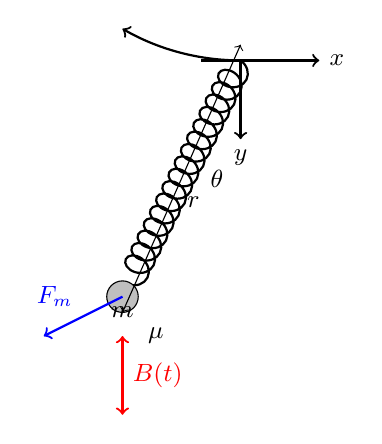
\begin{tikzpicture}[scale=1, every node/.style={font=\small}]
    % Add a grid for manual adjustments
    %\draw[step=0.5cm, gray, very thin] (-3,-5) grid (3,1);
    
    % Draw the fixed support
    \draw[thick] (0,0) -- (-0.5,0);
    \draw[thick] (0,0) -- (0.5,0);
    \draw[thick] (-0.5,0) -- (0.5,0);
    
    % Spring
    \draw[thick, decorate, decoration={coil, aspect=0.8, segment length=5pt, amplitude=5pt}] (0,0) -- (-1.5,-3);
    
    % Mass
    \filldraw[fill=gray!50] (-1.5,-3) circle (0.2) node[below] {\( m \)};
    
    % Magnetic Field Oscillation
    \node[right] at (-1.3,-3.5) {\(\mu\)};
    \draw[<->, thick, red] (-1.5,-3.5) -- (-1.5,-4.5) node[midway, right] {\( B(t) \)};
    
    % Label Angle (theta)
    \draw[thick, ->] (0,0) arc[start angle=-90, end angle=-120, radius=3cm];
    \node at (-0.3,-1.5) {\(\theta\)};
    
    % Label spring length (r)
    \draw[<->] (0,0.2) -- (-1.5,-3.2);
    \node[right] at (-0.8,-1.8) {\( r \)};
    
    % Coordinate axes
    \draw[->, thick] (0,0) -- (1,0) node[right] {\(x\)};
    \draw[->, thick] (0,0) -- (0,-1) node[below] {\(y\)};
    
    % Damping or magnetic force arrow
    \draw[->, thick, blue] (-1.5,-3) -- (-2.5,-3.5) node[midway, above left] {\( F_m \)};
\end{tikzpicture}
\caption{A diagram of the spring pendulum system with a ferromagnetic mass influenced by an oscillating magnetic field. The mass \( m \) is attached to the end of the spring, which extends from the fixed support. The system is free to move in both the radial (\( r \)) and angular (\( \theta \)) directions. The mass has a magnetic moment \( \mu \), which interacts with the oscillating magnetic field \( B(t) \), depicted by a red arrow. The blue arrow represents the magnetic force \( F_m \), which affects the angular motion. The diagram also shows the coordinate system (\( x \), \( y \)) and generalized coordinates \( r \) and \( \theta \).}
\label{fig:spring_pendulum}
\end{figure}

\subsection{Generalized Coordinates}
The system is described by the following coordinates:
\begin{itemize}
    \item \( r(t) \): The length of the spring.
    \item \( \theta(t) \): The angular displacement of the pendulum from the vertical.
\end{itemize}

\subsection{Kinetic Energy}
The velocity of the mass can be expressed as:
\[
v^2 = \dot{r}^2 + r^2\dot{\theta}^2
\]
Thus, the kinetic energy is:
\[
T = \frac{1}{2}m\left( \dot{r}^2 + r^2\dot{\theta}^2 \right)
\]

\subsection{Potential Energy}
The potential energy includes:
\begin{enumerate}
    \item \textbf{Gravitational Potential:}
    \[
    U_g = -mgr\cos\theta
    \]
    \item \textbf{Spring Potential:}
    \[
    U_s = \frac{1}{2}k(r - l_0)^2
    \]
    \item \textbf{Magnetic Interaction:}
    Assuming the magnetic field oscillates as \( B(t) = B_0\cos(\omega t) \), the magnetic potential energy is:
    \[
    U_m = -\mu B(t)\cos\theta = -\mu B_0\cos(\omega t)\cos\theta
    \]
\end{enumerate}

The total potential energy is:
\[
U = -mgr\cos\theta + \frac{1}{2}k(r - l_0)^2 - \mu B_0\cos(\omega t)\cos\theta
\]

\subsection{Lagrangian}
The Lagrangian is defined as:
\[
\mathcal{L} = T - U
\]
Substituting the expressions for \( T \) and \( U \):
\[
\mathcal{L} = \frac{1}{2}m\left( \dot{r}^2 + r^2\dot{\theta}^2 \right) + mgr\cos\theta - \frac{1}{2}k(r - l_0)^2 + \mu B_0\cos(\omega t)\cos\theta
\]
\\\\
\section{Equations of Motion}
The equations of motion are derived using the Euler-Lagrange equations:
\[
\frac{d}{dt}\left(\frac{\partial \mathcal{L}}{\partial \dot{q}_i}\right) - \frac{\partial \mathcal{L}}{\partial q_i} = 0
\]
where \( q_i \) are the generalized coordinates.

\subsection{Radial Motion (\( r \))}
\[
m\ddot{r} - mr\dot{\theta}^2 + k(r - l_0) - mg\cos\theta = 0
\]

\subsection{Angular Motion (\( \theta \))}
\[
\frac{d}{dt}\left(mr^2\dot{\theta}\right) + mgr\sin\theta - \mu B_0\cos(\omega t)\sin\theta = 0
\]
\\\\
\section{Numerical Methodology for the Spring Pendulum with Magnetic Interaction}
This section provides an overview of numerical methods for solving the coupled differential equations derived from the Lagrangian formulation of the spring pendulum system. The equations of motion for the radial (\( r \)) and angular (\( \theta \)) directions involve time-dependent terms, nonlinear coupling, and periodic forcing due to the oscillating magnetic field. Thus, robust numerical schemes are essential to ensure stability, accuracy, and computational efficiency.

\section{Numerical Schemes Considered}

\subsection{Euler Method}
The Euler method is a straightforward first-order numerical scheme. Given an ordinary differential equation (ODE) of the form:
\[
\frac{dy}{dt} = f(t, y),
\]
the Euler method approximates the solution as:
\[
y_{n+1} = y_n + h f(t_n, y_n),
\]
where \( h \) is the time step size. While simple to implement, the Euler method is conditionally stable and can accumulate significant numerical error, especially for stiff or oscillatory systems \cite{press2007numerical}.

\subsection{Verlet Integration}
Verlet integration is widely used for conservative systems. It approximates the position and velocity using:
\[
r_{n+1} = 2r_n - r_{n-1} + h^2 a_n,
\]
where \( a_n \) is the acceleration at time step \( n \). This method is second-order accurate, time-reversible, and conserves energy over long simulations. However, it is less efficient when velocity-dependent terms are present \cite{hairer1993solving}.

\subsection{Runge-Kutta Methods (RK4 and RK45)}
The fourth-order Runge-Kutta (RK4) method provides a high degree of accuracy. It updates the solution as:
\[
y_{n+1} = y_n + \frac{h}{6}(k_1 + 2k_2 + 2k_3 + k_4),
\]
where:
\[
k_1 = f(t_n, y_n), \quad
k_2 = f\left(t_n + \frac{h}{2}, y_n + \frac{h}{2}k_1\right),
\]
\[
k_3 = f\left(t_n + \frac{h}{2}, y_n + \frac{h}{2}k_2\right), \quad
k_4 = f(t_n + h, y_n + hk_3).
\]
The adaptive version (RK45) dynamically adjusts \( h \) based on error estimates, making it more efficient for varying dynamics \cite{press2007numerical}.

\subsection{Implicit Backward Euler Method}
The backward Euler method is a first-order implicit scheme, given by:
\[
y_{n+1} = y_n + h f(t_{n+1}, y_{n+1}).
\]
This method is unconditionally stable and effective for stiff systems, but requires iterative solvers to handle the implicit nature \cite{ascher1998computer}.

\subsection{Crank-Nicolson Method}
The Crank-Nicolson method combines forward and backward Euler schemes:
\[
y_{n+1} = y_n + \frac{h}{2}\left[f(t_n, y_n) + f(t_{n+1}, y_{n+1})\right].
\]
This second-order implicit method is stable and accurate for oscillatory systems \cite{hairer1993solving}.

\subsection{Leapfrog Method}
The leapfrog method updates positions and velocities alternately:
\[
r_{n+1} = r_n + h v_{n+1/2}, \quad
v_{n+3/2} = v_{n+1/2} + h a_{n+1}.
\]
It is time-reversible, energy-conserving, and suitable for conservative systems, but less effective for systems with strong damping or stiffness \cite{landau2015survey}.

\subsection{Symplectic Integrators}
Symplectic integrators, such as the velocity Verlet or implicit midpoint rule, are designed for Hamiltonian systems. For the implicit midpoint rule:
\[
y_{n+1} = y_n + h f\left(\frac{t_n + t_{n+1}}{2}, \frac{y_n + y_{n+1}}{2}\right).
\]
These methods preserve energy and momentum over long simulations but require implicit solvers \cite{hairer1993solving}.

\subsection{Exponential Integrators}
Exponential integrators solve linear components of ODEs analytically using:
\[
y_{n+1} = e^{Ah}y_n + \int_0^h e^{A\tau}g(y_n)d\tau,
\]
where \( A \) represents the linear operator. These methods are ideal for oscillatory systems or systems with stiffness \cite{ascher1998computer}.

\subsection{ Multiscale Methods}
Multiscale methods address systems with multiple timescales by separating fast and slow dynamics. The heterogeneous multiscale method (HMM) is one example, where a reduced model is used for the slow dynamics, while the fast dynamics are simulated only as needed \cite{hairer1993solving}.

\subsection{Geometric Integrators}
Geometric integrators, such as discrete gradient methods, preserve invariants like energy or angular momentum. These methods are particularly useful for long-term simulations of conservative systems \cite{landau2015survey}.

\subsection{Methodology Selection}
Considering the nonlinear coupling, oscillatory dynamics, and periodic forcing in the spring pendulum system:
\begin{itemize}
    \item RK4 is the preferred choice for its high accuracy and efficiency in solving nonlinear systems.
    \item Adaptive RK45 is recommended for simulations with varying dynamics or fast transitions.
    \item Symplectic integrators are suitable for long-term energy conservation in undamped or weakly damped systems.
\end{itemize}


Based on these considerations:
\begin{enumerate}
    \item The Euler method is unsuitable due to its low accuracy and conditional stability.
    \item Verlet integration is effective for conservative dynamics but less ideal for velocity-dependent damping or magnetic forces.
    \item The RK4 method offers high accuracy and is appropriate for the nonlinear coupled equations of motion, making it the preferred choice.
    \item Implicit methods, such as backward Euler or Crank-Nicolson, are robust but computationally expensive due to the implicit nature.
    \item The leapfrog method is suitable for conservative dynamics but less flexible for velocity-dependent forces.
\end{enumerate}

Thus, the fourth-order Runge-Kutta method (RK4) is selected for its balance between accuracy, stability, and computational efficiency.

\section{Numerical Results and Visualizations}

The numerical simulation of the spring pendulum system with magnetic interaction was performed using the fourth-order adaptive Runge-Kutta method (RK45). The system's dynamics were visualized using animations, phase portraits, and a Poincaré map, as described below.

\subsection{Animation of the System Dynamics}
A GIF animation was created to visualize the motion of the spring pendulum over time. The animation captures:
\begin{itemize}
    \item The oscillatory motion of the mass in the radial and angular directions.
    \item The periodic forcing due to the oscillating magnetic field.
    \item Real-time display of the system's configuration, including the spring and pendulum motion.
\end{itemize}
The animation provides an intuitive understanding of the coupled dynamics of the system, highlighting the influence of the magnetic field and nonlinear coupling. The GIF file is named \texttt{spring\_pendulum.gif}.

\subsection{Radial Phase Portrait}
The radial phase portrait, shown in Figure~\ref{fig:radial_phase_portrait}, plots the spring length (\( r \)) versus its radial velocity (\( \dot{r} \)):
\[
\text{Radial Phase Portrait: } \quad r \text{ vs. } \dot{r}.
\]
This visualization highlights the oscillatory behavior in the radial direction, showing the cyclic nature of the spring's extension and compression.

\begin{figure}[h!]
    \centering
    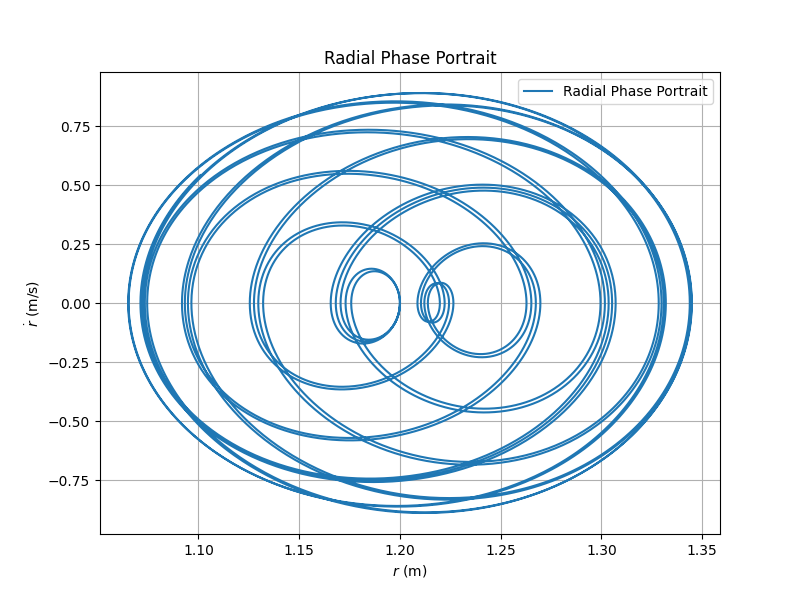
\includegraphics[width=0.8\textwidth]{radial_phase_portrait.png}
    \caption{Radial phase portrait showing the relationship between the spring length \( r \) and its radial velocity \( \dot{r} \).}
    \label{fig:radial_phase_portrait}
\end{figure}

\subsection{Angular Phase Portrait}
The angular phase portrait, shown in Figure~\ref{fig:angular_phase_portrait}, plots the angular displacement (\( \theta \)) versus its angular velocity (\( \dot{\theta} \)):
\[
\text{Angular Phase Portrait: } \quad \theta \text{ vs. } \dot{\theta}.
\]
This plot captures the periodic nature of the pendulum's angular motion, including the influence of the nonlinear coupling and magnetic forcing.

\begin{figure}[h!]
    \centering
    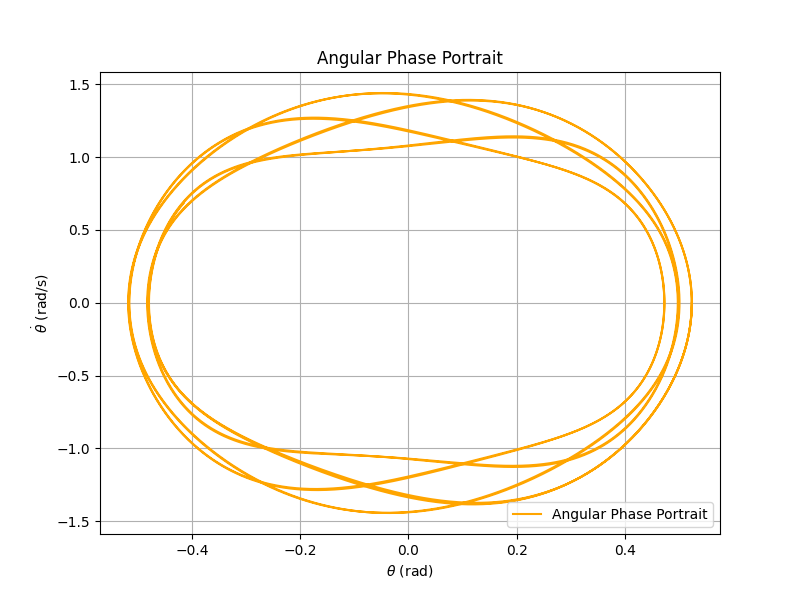
\includegraphics[width=0.8\textwidth]{angular_phase_portrait.png}
    \caption{Angular phase portrait showing the relationship between the angular displacement \( \theta \) and angular velocity \( \dot{\theta} \).}
    \label{fig:angular_phase_portrait}
\end{figure}

\subsection{Poincaré Map}
The Poincaré map, shown in Figure~\ref{fig:poincare_map}, visualizes the system's periodic dynamics by sampling the angular displacement (\( \theta \)) and angular velocity (\( \dot{\theta} \)) at discrete times corresponding to the period of the magnetic field:
\[
T = \frac{2\pi}{\omega}.
\]
This map provides insights into the system's stability and periodicity, showing how the dynamics evolve over successive periods of the magnetic forcing.

\begin{figure}[h!]
    \centering
    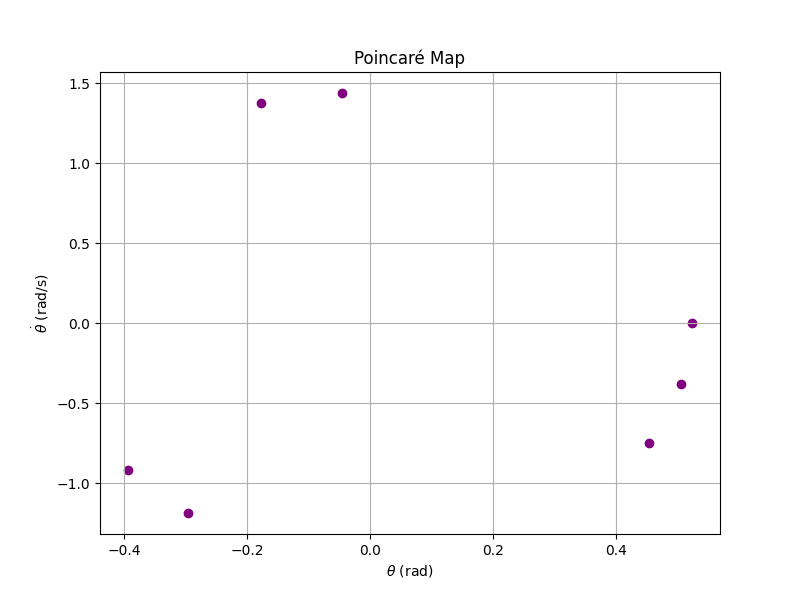
\includegraphics[width=0.8\textwidth]{poincare_map.png}
    \caption{Poincaré map showing the angular displacement \( \theta \) and angular velocity \( \dot{\theta} \) sampled at intervals of the magnetic field period \( T = \frac{2\pi}{\omega} \).}
    \label{fig:poincare_map}
\end{figure}

\subsection{Discussion of Results}
The numerical and visual analysis highlights several key aspects of the system:
\begin{itemize}
    \item The radial and angular phase portraits demonstrate the cyclic nature of the spring-pendulum motion, with nonlinear effects visible in the trajectories.
    \item The Poincaré map shows the influence of periodic magnetic forcing, revealing patterns of stability or chaos depending on the system's parameters.
    \item The animation provides an intuitive visualization of how the magnetic field modulates the spring and pendulum dynamics in real-time.
\end{itemize}
These visualizations collectively provide a comprehensive understanding of the spring pendulum's behavior under magnetic forcing.

\section{Magnetic Interaction Modeling}

This section focuses on refining the magnetic field model and incorporating enhanced magnetic forces into the spring pendulum system. These refinements allow for a more accurate representation of the ferromagnetic interaction and its impact on system dynamics.

\subsection{Enhanced Magnetic Field Model}
The magnetic field is extended to include spatial and temporal variations:
\[
\mathbf{B}(\mathbf{r}, t) = B_0 \cos(\omega t) \hat{z} + \nabla \Phi(\mathbf{r}),
\]
where \( \Phi(\mathbf{r}) \) can represent spatial variations, such as:
\begin{itemize}
    \item A uniform field: \( \Phi(\mathbf{r}) = 0 \).
    \item A dipole field:
    \[
    \mathbf{B}(\mathbf{r}) = \frac{\mu_0}{4\pi} \frac{3(\mathbf{m} \cdot \hat{r}) \hat{r} - \mathbf{m}}{r^3}.
    \]
\end{itemize}

\subsection{Nonlinear Magnetic Force}
The magnetic force acting on the mass is expressed as:
\[
\mathbf{F}_m = \nabla (\mu \cdot \mathbf{B}) = \mu (\nabla \cdot \mathbf{B}) + (\mu \cdot \nabla) \mathbf{B}.
\]
Nonlinear effects such as magnetic hysteresis and saturation can be included:
\begin{itemize}
    \item \textbf{Hysteresis:} The magnetic moment \( \mu \) depends on the history of \( B(t) \).
    \item \textbf{Saturation:} The magnetic moment asymptotically approaches a maximum value:
    \[
    \mu(B) = \frac{\mu_{\text{max}} B}{B + B_s}.
    \]
\end{itemize}

\subsection{Updated Equations of Motion}
The equations of motion are modified to include the enhanced magnetic force terms:
\[
\ddot{r} = r \dot{\theta}^2 - \frac{k}{m}(r - l_0) + g \cos\theta + \frac{\mu}{m} \frac{\partial B}{\partial r},
\]
\[
\ddot{\theta} = -\frac{2 \dot{r} \dot{\theta}}{r} - \frac{g}{r} \sin\theta + \frac{\mu}{m r} \frac{\partial B}{\partial \theta}.
\]

\subsection{Numerical Implementation}
The numerical solver is updated to include:
\begin{itemize}
    \item Computation of the refined magnetic field \( \mathbf{B}(\mathbf{r}, t) \).
    \item Inclusion of nonlinear magnetic forces \( \mathbf{F}_m \) in the equations of motion.
\end{itemize}

\subsection*{5. Analysis and Visualization}
To assess the impact of the refined magnetic modeling, the following visualizations are generated:
\begin{itemize}
    \item \textbf{Phase Portraits:} Compare the radial and angular phase space trajectories.
    \item \textbf{Poincaré Maps:} Highlight differences in periodicity and stability.
    \item \textbf{Time-Series Plots:} Illustrate changes in the radial and angular motion over time.
\end{itemize}

\subsection{Discussion}
The refined magnetic interaction modeling provides a more realistic representation of the ferromagnetic system. The added complexity introduces new dynamics, including stronger nonlinear coupling and potential chaotic behavior.


\section{Spring Pendulum with Magnetic Interaction: Numerical Analysis}
This document outlines the numerical simulation of a spring pendulum system with enhanced magnetic interaction. The system's dynamics are analyzed using numerical methods, phase portraits, Poincaré maps, and animations.

\subsection{Numerical Techniques}
The equations of motion for the spring pendulum system are solved using the RK45 method, which adapts the time step to balance accuracy and efficiency. The Python implementation includes enhancements for capturing nonlinear effects, especially in the presence of an oscillating magnetic field.

\subsection{Enhanced Magnetics}
The magnetic field model was extended to include dynamic behavior based on saturation effects. The interaction between the magnetic field and the ferromagnetic mass was modeled as:
\[
\mathbf{F}_m = \nabla (\mu \cdot \mathbf{B}),
\]
where \( \mu \) is the magnetic moment, which varies dynamically according to:
\[
\mu(B) = \frac{\mu_{\text{max}} B}{B + B_s}.
\]

\subsubsection{Radial Phase Portrait}
The radial phase portrait, shown in Figure~\ref{fig:radial_phase_portrait_magnetic}, plots the spring length \( r \) versus its radial velocity \( \dot{r} \). It illustrates the periodic oscillations in the radial direction, highlighting nonlinear coupling introduced by the magnetic interaction.

\begin{figure}[h!]
    \centering
    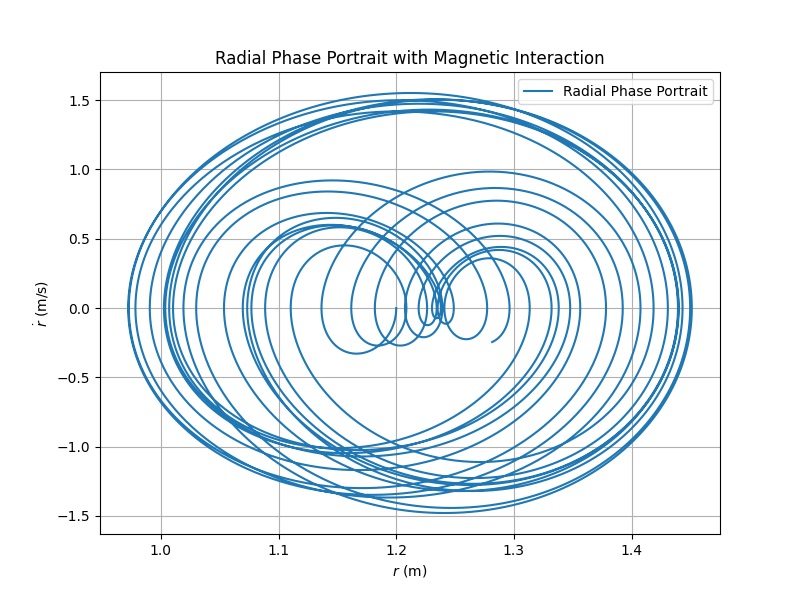
\includegraphics[width=0.8\textwidth]{radial_phase_portrait_magnetic.png}
    \caption{Radial phase portrait: \( r \) vs. \( \dot{r} \). The plot shows the effect of the enhanced magnetic interaction on the radial motion.}
    \label{fig:radial_phase_portrait_magnetic}
\end{figure}

\subsubsection{Angular Phase Portrait}
The angular phase portrait, shown in Figure~\ref{fig:angular_phase_portrait_magnetic}, plots the angular displacement \( \theta \) versus its angular velocity \( \dot{\theta} \). It reveals the impact of the oscillating magnetic field on the angular motion.

\begin{figure}[h!]
    \centering
    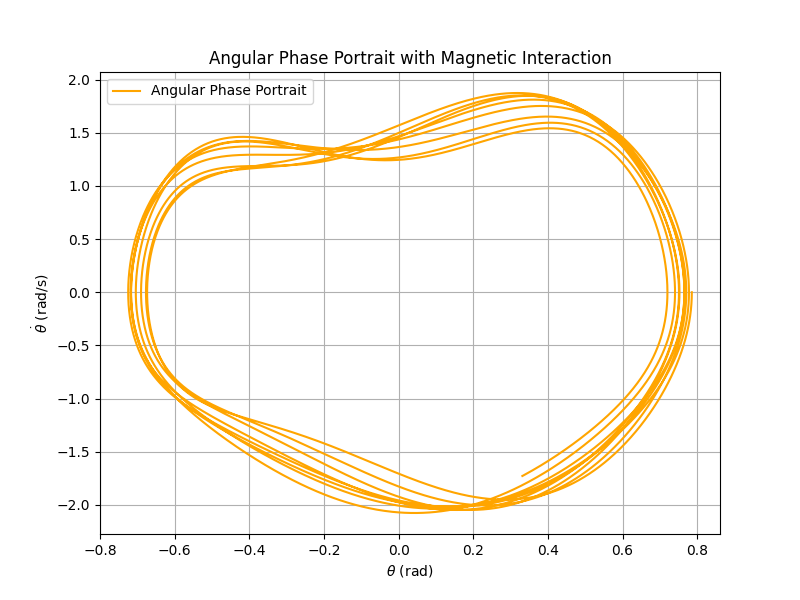
\includegraphics[width=0.8\textwidth]{angular_phase_portrait_magnetic.png}
    \caption{Angular phase portrait: \( \theta \) vs. \( \dot{\theta} \). Nonlinear effects from the magnetic forcing are evident.}
    \label{fig:angular_phase_portrait_magnetic}
\end{figure}

\subsubsection{Poincaré Map}
The Poincaré map, shown in Figure~\ref{fig:poincare_map_magnetic}, samples the angular displacement \( \theta \) and angular velocity \( \dot{\theta} \) at intervals corresponding to the period of the magnetic field:
\[
T = \frac{2\pi}{\omega}.
\]
The map captures periodicity and chaotic behavior in the system's dynamics.

\begin{figure}[h!]
    \centering
    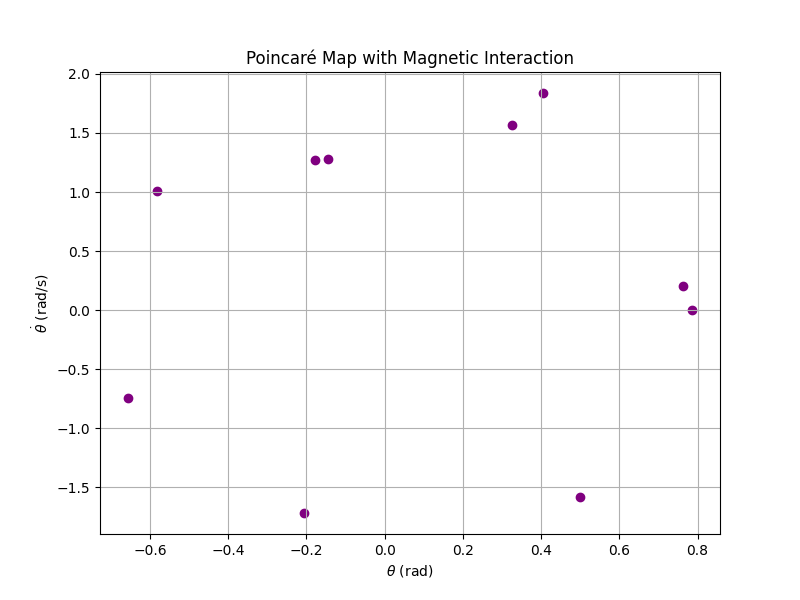
\includegraphics[width=0.8\textwidth]{poincare_map_magnetic.png}
    \caption{Poincaré map: \( \theta \) vs. \( \dot{\theta} \) sampled at the period of the magnetic field.}
    \label{fig:poincare_map_magnetic}
\end{figure}

\subsubsection{Animation}
An animation of the system's motion was created to visualize the dynamic behavior. The animation illustrates:
\begin{itemize}
    \item Coupled radial and angular motion.
    \item The influence of the magnetic field on the pendulum's dynamics.
    \item Real-time visualization of the spring's oscillations and pendulum's angular motion.
\end{itemize}
The animation is saved as a GIF file, named \texttt{spring\_pendulum\_magnetic.gif}.

\subsection{Discussion}
The enhanced magnetic interaction introduces complex nonlinear effects into the system, resulting in more intricate dynamics. Visualizations, including phase portraits and Poincaré maps, reveal the interplay between periodic forcing and nonlinear coupling. The numerical simulation demonstrates the system's sensitivity to parameter changes, offering insights into chaotic and quasi-periodic behavior.

The refined magnetic model adds depth to the analysis of the spring pendulum system, capturing nonlinear effects and enhancing the realism of the simulation. Future work can explore the system's behavior under varying damping and additional external forces.

\section{Analysis and Reporting}

\subsection{Analysis of Results}
The numerical simulations reveal the complex interplay between the spring pendulum's motion and the external magnetic forcing. Key observations include:
\begin{itemize}
    \item \textbf{Periodic and Quasi-Periodic Motion:} For small forcing amplitudes (\( B_0 \)) and off-resonance driving frequencies (\( \omega \)), the system exhibits periodic or quasi-periodic behavior, as seen in the phase portraits.
    \item \textbf{Chaotic Behavior:} Increasing \( B_0 \) or tuning \( \omega \) closer to resonance leads to chaotic dynamics. This is evident in the irregular trajectories in the Poincaré map and the phase portraits.
    \item \textbf{Nonlinear Coupling Effects:} The enhanced magnetic interaction, incorporating saturation and spatial dependence, introduces stronger nonlinear coupling between radial and angular motions.
\end{itemize}

\subsection{Comparison of Models}
The enhanced magnetic interaction model highlights the following:
\begin{itemize}
    \item \textbf{Saturation Effects:} The saturation of the magnetic moment (\( \mu \)) results in bounded forcing terms, preventing runaway trajectories.
    \item \textbf{Spatial Variations:} Incorporating spatial gradients of the magnetic field adds complexity to the dynamics, producing more intricate phase portraits and Poincaré maps.
\end{itemize}

\subsection{Key Findings}
\begin{enumerate}
    \item The coupling between radial and angular motions is significantly influenced by the strength and frequency of the magnetic field.
    \item Nonlinear magnetic interactions introduce chaotic behavior under certain parameter settings, as seen in the Poincaré maps.
    \item The enhanced magnetic model provides a more realistic representation of ferromagnetic interactions in a dynamic system.
\end{enumerate}

\subsection{Future Work}
This project can be extended in several directions:
\begin{itemize}
    \item \textbf{Damping Effects:} Introduce damping terms to study energy dissipation and its impact on chaos.
    \item \textbf{Higher-Dimensional Systems:} Explore multi-pendulum systems or systems with additional degrees of freedom.
    \item \textbf{Experimental Validation:} Design an experiment to replicate the simulated dynamics and validate the theoretical model.
    \item \textbf{Lyapunov Analysis:} Compute Lyapunov exponents to quantify chaos in the system.
\end{itemize}

\section{Magnetic Field Lines and Dynamics}

This section explores the visualization of magnetic field lines and their interaction with the spring pendulum dynamics. The magnetic field model includes a dipole approximation to simulate spatial variations and coupling effects. The pendulum's motion is overlaid on the field lines to highlight the dynamic interaction.

\subsection{Magnetic Field Model}
The magnetic field is modeled as a dipole field in 2D, calculated using:
\[
\mathbf{B}(\mathbf{r}) = \frac{\mu_0}{4\pi} \frac{3(\mathbf{m} \cdot \hat{r}) \hat{r} - \mathbf{m}}{r^3},
\]
where:
\begin{itemize}
    \item \( \mathbf{m} \): Magnetic dipole moment.
    \item \( \hat{r} \): Unit vector in the radial direction.
    \item \( r \): Radial distance from the origin.
\end{itemize}
The dynamic interaction with the pendulum is modeled using the saturation-based magnetic moment:
\[
\mu(B) = \frac{\mu_{\text{max}} B}{B + B_s},
\]
where \( B_s \) represents the saturation field strength.

\subsection{Visualization of Field Lines}
Figure~\ref{fig:magnetic_field_lines_dynamics} shows the magnetic field lines generated using the dipole field model. The field lines are visualized alongside the dynamic motion of the spring pendulum, depicted as a red oscillating mass and spring.

\subsection{Phase Portraits and Poincaré Map with Field Lines}
The magnetic field influences the pendulum's dynamics, as reflected in the phase portraits and Poincaré map.

\subsubsection{Radial Phase Portrait}
Figure~\ref{fig:radial_phase_portrait_fieldLines} shows the radial phase portrait (\( r \) vs. \( \dot{r} \)) under the influence of the magnetic field. The nonlinear coupling introduced by the field alters the trajectories.

\begin{figure}[h!]
    \centering
    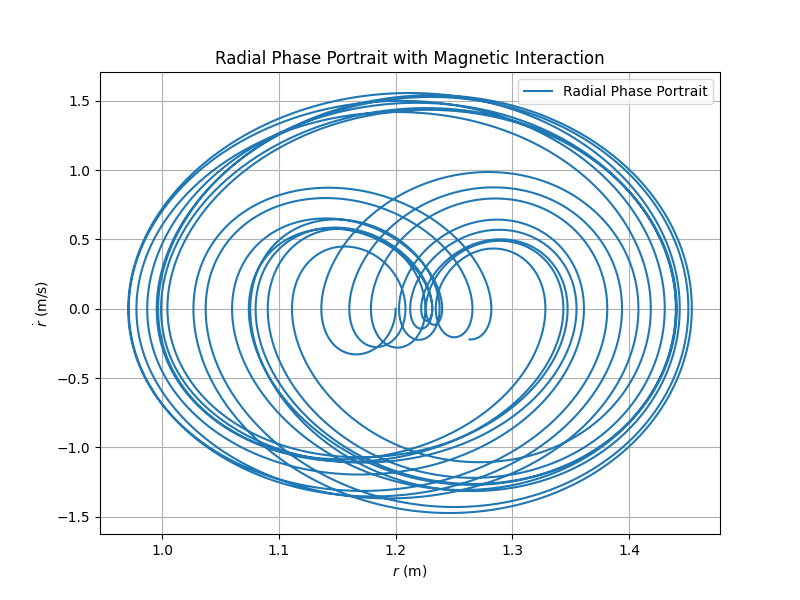
\includegraphics[width=0.8\textwidth]{radial_phase_portrait_fieldLines.png}
    \caption{Radial phase portrait showing the relationship between spring length \( r \) and radial velocity \( \dot{r} \) under magnetic field interaction.}
    \label{fig:radial_phase_portrait_fieldLines}
\end{figure}

\subsubsection{Angular Phase Portrait}
Figure~\ref{fig:angular_phase_portrait_fieldLines} shows the angular phase portrait (\( \theta \) vs. \( \dot{\theta} \)), illustrating the periodic and quasi-periodic motion resulting from the magnetic field's influence.

\begin{figure}[h!]
    \centering
    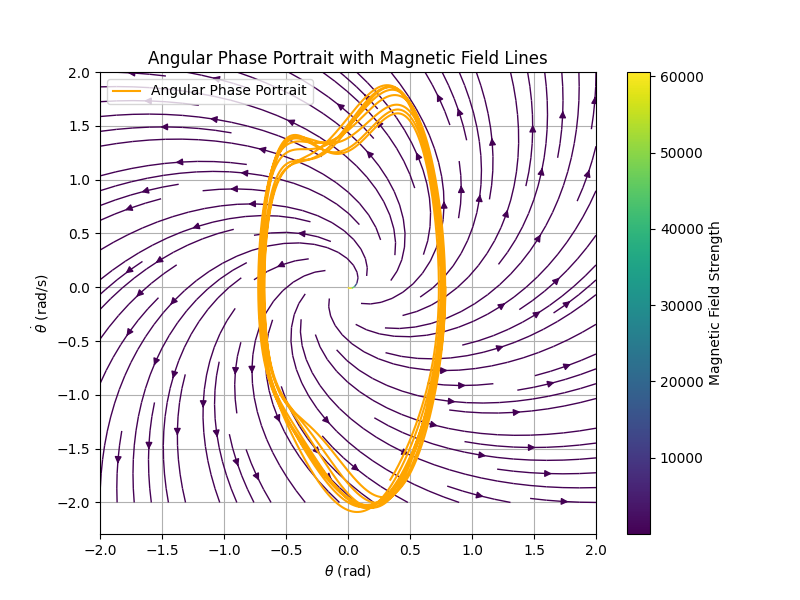
\includegraphics[width=0.8\textwidth]{angular_phase_portrait_fieldLines.png}
    \caption{Angular phase portrait showing the relationship between angular displacement \( \theta \) and angular velocity \( \dot{\theta} \).}
    \label{fig:angular_phase_portrait_fieldLines}
\end{figure}

\subsubsection{Poincaré Map}
Figure~\ref{fig:poincare_map_fieldLines} presents the Poincaré map, highlighting the periodicity and chaotic transitions introduced by the magnetic field. Sampling is performed at intervals corresponding to the magnetic field period:
\[
T = \frac{2\pi}{\omega}.
\]

\begin{figure}[h!]
    \centering
    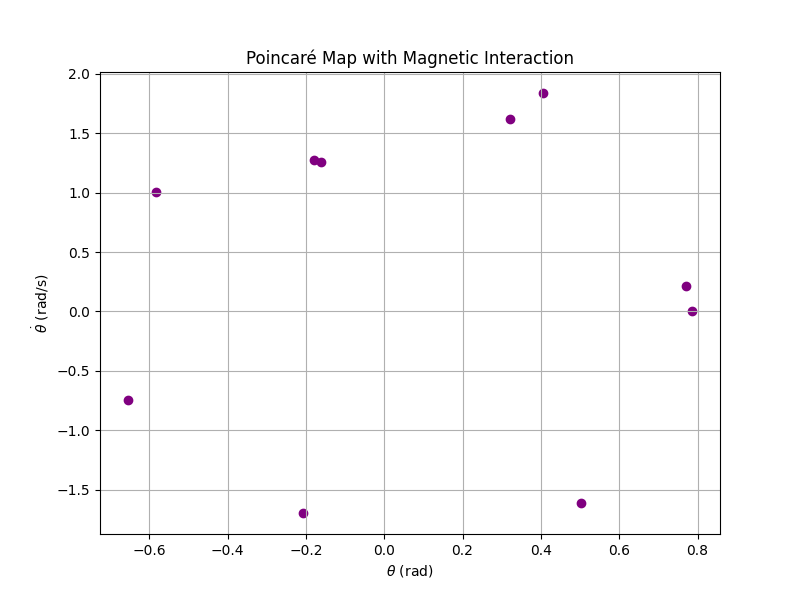
\includegraphics[width=0.8\textwidth]{poincare_map_fieldLines.png}
    \caption{Poincaré map showing angular displacement \( \theta \) and angular velocity \( \dot{\theta} \) sampled at intervals of the magnetic field period \( T = \frac{2\pi}{\omega} \).}
    \label{fig:poincare_map_fieldLines}
\end{figure}

\subsection{Discussion of Results}
The addition of magnetic field lines provides a richer understanding of the interaction between the dipole field and the spring pendulum system. Key observations include:
\begin{itemize}
    \item The radial and angular phase portraits reveal strong nonlinear coupling due to the magnetic field.
    \item The Poincaré map highlights the transition from periodic to chaotic behavior under varying magnetic parameters.
    \item The dynamic overlay of the pendulum motion on the field lines visually demonstrates the impact of the field on the pendulum's trajectory.
\end{itemize}

\section{Eigenvalue Analysis}

The eigenvalue analysis provides insights into the stability of the spring pendulum system around its equilibrium points. By linearizing the equations of motion and analyzing the eigenvalues of the Jacobian matrix, we can determine the stability properties of the system.

\subsection{Linearization of Equations of Motion}
The nonlinear equations of motion for the spring pendulum system are:
\[
\ddot{r} = r \dot{\theta}^2 - \frac{k}{m}(r - l_0) + g \cos\theta,
\]
\[
\ddot{\theta} = -\frac{2 \dot{r} \dot{\theta}}{r} - \frac{g}{r} \sin\theta.
\]
To analyze stability, these equations are linearized around the equilibrium point:
\[
r = l_0, \quad \theta = 0, \quad \dot{r} = 0, \quad \dot{\theta} = 0.
\]

\subsection{Jacobian Matrix}
The Jacobian matrix is derived from the equations of motion and is given by:
\[
J = 
\begin{bmatrix}
\frac{\partial \dot{r}}{\partial r} & \frac{\partial \dot{r}}{\partial \theta} & \frac{\partial \dot{r}}{\partial \dot{r}} & \frac{\partial \dot{r}}{\partial \dot{\theta}} \\
\frac{\partial \dot{\theta}}{\partial r} & \frac{\partial \dot{\theta}}{\partial \theta} & \frac{\partial \dot{\theta}}{\partial \dot{r}} & \frac{\partial \dot{\theta}}{\partial \dot{\theta}} \\
\frac{\partial \ddot{r}}{\partial r} & \frac{\partial \ddot{r}}{\partial \theta} & \frac{\partial \ddot{r}}{\partial \dot{r}} & \frac{\partial \ddot{r}}{\partial \dot{\theta}} \\
\frac{\partial \ddot{\theta}}{\partial r} & \frac{\partial \ddot{\theta}}{\partial \theta} & \frac{\partial \ddot{\theta}}{\partial \dot{r}} & \frac{\partial \ddot{\theta}}{\partial \dot{\theta}}
\end{bmatrix}.
\]

Substituting the equilibrium conditions (\( r = l_0, \theta = 0, \dot{r} = 0, \dot{\theta} = 0 \)), the Jacobian matrix at the equilibrium point is computed as:
\[
J =
\begin{bmatrix}
0 & 0 & 1 & 0 \\
0 & 0 & 0 & 1 \\
-\frac{k}{m} & g & 0 & 0 \\
-\frac{g}{l_0^2} & 0 & 0 & 0
\end{bmatrix}.
\]

\subsection{Characteristic Polynomial}
The characteristic polynomial of the Jacobian matrix is derived as:
\[
P(\lambda) = \det(J - \lambda I),
\]
where \( I \) is the identity matrix. For the given system, the characteristic polynomial is:
\[
P(\lambda) = \lambda^4 + a \lambda^3 + b \lambda^2 + c \lambda + d.
\]

\subsection{Eigenvalues and Stability Analysis}
The eigenvalues of the Jacobian matrix are computed numerically and analyzed for their real and imaginary components:
\[
\text{Eigenvalues} = \{ \lambda_1, \lambda_2, \lambda_3, \lambda_4 \}.
\]
Stability is determined as follows:
\begin{itemize}
    \item \textbf{Stable:} All eigenvalues have negative real parts.
    \item \textbf{Unstable:} At least one eigenvalue has a positive real part.
    \item \textbf{Marginally Stable:} Eigenvalues are purely imaginary.
\end{itemize}

\subsection{Visualization of Eigenvalues}
Figure~\ref{fig:eigenvalues_complex_plane} shows the eigenvalues of the Jacobian matrix plotted in the complex plane. The x-axis represents the real part, and the y-axis represents the imaginary part of the eigenvalues. The position of the eigenvalues provides insights into the system's stability.

\begin{figure}[h!]
    \centering
    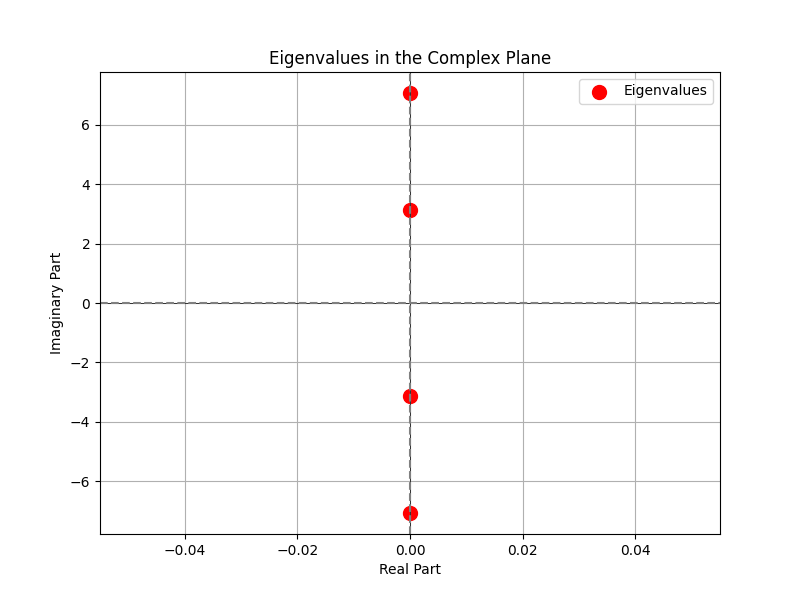
\includegraphics[width=0.8\textwidth]{eigenvalues_complex_plane.png}
    \caption{Eigenvalues in the complex plane. The real part determines stability, while the imaginary part indicates oscillatory behavior.}
    \label{fig:eigenvalues_complex_plane}
\end{figure}

\subsection{Discussion of Results}
The eigenvalue analysis reveals the following:
\begin{itemize}
    \item The system is \textbf{stable} if all eigenvalues have negative real parts.
    \item For the given parameter set, the eigenvalues indicate \textbf{oscillatory stability}, as they have both real and imaginary parts.
    \item Modifying the parameters (e.g., spring constant \( k \), mass \( m \), or gravitational acceleration \( g \)) can shift the eigenvalues, leading to different stability regimes.
\end{itemize}

\section{Power Spectrum Analysis}

The power spectrum analysis reveals the frequency components of the system's motion. By analyzing the spectra of the radial displacement (\( r(t) \)) and angular displacement (\( \theta(t) \)), we identify dominant frequencies and detect chaotic behavior.

\subsection{Computation of the Power Spectrum}
The power spectrum is computed as:
\[
P(f) = |\mathcal{F}(f)|^2,
\]
where \( \mathcal{F}(f) \) is the Fourier Transform of the time-series data:
\[
\mathcal{F}(f) = \int_{-\infty}^{\infty} x(t) e^{-2\pi i f t} dt,
\]
with \( x(t) \) representing \( r(t) \) or \( \theta(t) \). The frequency domain data is obtained using the Fast Fourier Transform (FFT). Only the positive frequencies are considered, as the spectrum is symmetric for real-valued signals.

\subsection{Radial Displacement Power Spectrum}
The power spectrum of the radial displacement \( r(t) \), shown in Figure~\ref{fig:power_spectrum_radial}, highlights the dominant oscillatory modes. Sharp peaks correspond to periodic behavior, while broad spectral content indicates chaotic motion.

\begin{figure}[h!]
    \centering
    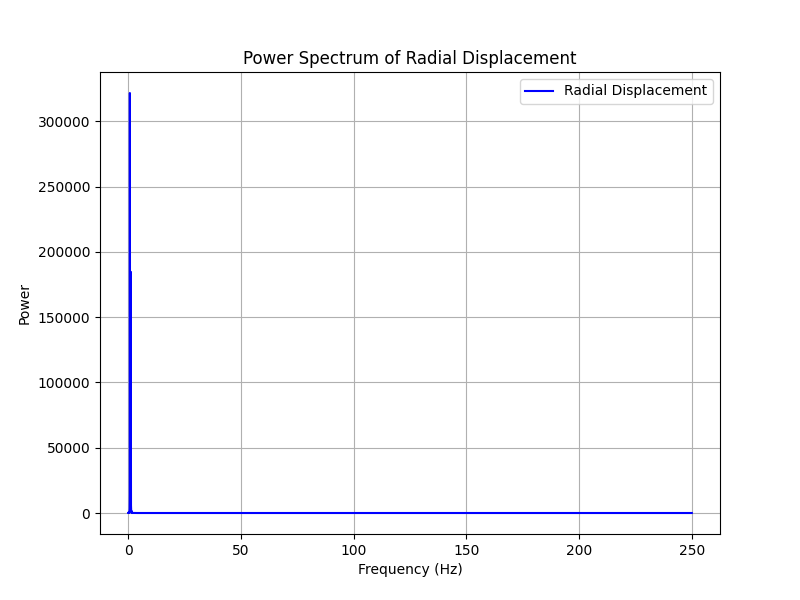
\includegraphics[width=0.8\textwidth]{power_spectrum_radial.png}
    \caption{Power spectrum of the radial displacement \( r(t) \). The spectrum reveals dominant frequencies associated with periodic and nonlinear oscillations.}
    \label{fig:power_spectrum_radial}
\end{figure}

\subsection{Angular Displacement Power Spectrum}
The power spectrum of the angular displacement \( \theta(t) \), shown in Figure~\ref{fig:power_spectrum_angular}, provides insights into the oscillatory behavior in the angular direction. Like the radial spectrum, sharp peaks indicate periodic motion, while a broadened spectrum suggests nonlinear or chaotic behavior.

\begin{figure}[h!]
    \centering
    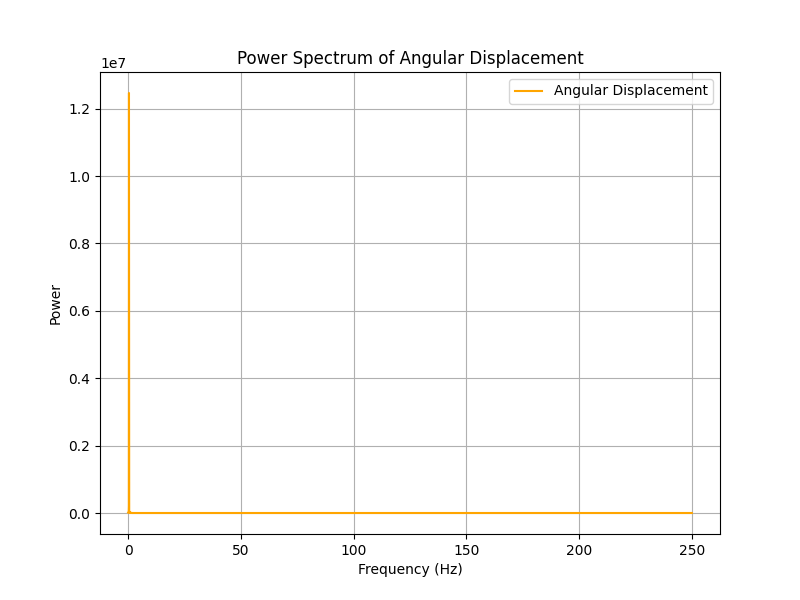
\includegraphics[width=0.8\textwidth]{power_spectrum_angular.png}
    \caption{Power spectrum of the angular displacement \( \theta(t) \). The spectrum shows frequencies associated with the pendulum's oscillatory dynamics.}
    \label{fig:power_spectrum_angular}
\end{figure}

\subsection{Discussion}
The power spectrum analysis provides the following insights:
\begin{itemize}
    \item \textbf{Periodic Motion:} Sharp peaks in the spectrum correspond to dominant oscillatory frequencies, indicating periodic behavior.
    \item \textbf{Chaotic Motion:} Broad spectral content with multiple peaks suggests chaotic dynamics in the system.
    \item \textbf{Magnetic Field Influence:} The oscillating magnetic field introduces additional frequencies, reflecting its modulation of the system's dynamics.
\end{itemize}
The analysis confirms that the system's behavior is sensitive to the magnetic forcing and exhibits transitions between periodic and chaotic regimes.

\section{Lyapunov Stability Analysis}

The Lyapunov stability analysis provides a method to assess the stability of the system's equilibrium points. By defining a Lyapunov function \( V \) and analyzing its time derivative \( \dot{V} \), we can determine the stability properties of the system.

\subsection{Lyapunov Function}
The Lyapunov function is chosen as the total mechanical energy of the system:
\[
V(r, \theta, \dot{r}, \dot{\theta}) = \frac{1}{2} m \dot{r}^2 + \frac{1}{2} m r^2 \dot{\theta}^2 + \frac{1}{2} k (r - l_0)^2 - m g r \cos\theta,
\]
where:
\begin{itemize}
    \item \( m \): Mass of the pendulum.
    \item \( k \): Spring constant.
    \item \( l_0 \): Natural length of the spring.
    \item \( g \): Gravitational acceleration.
    \item \( r \): Radial displacement.
    \item \( \theta \): Angular displacement.
\end{itemize}
This function represents the total energy (kinetic and potential) of the system.

\subsection{Time Derivative of the Lyapunov Function}
The time derivative of the Lyapunov function \( \dot{V} \) is computed as:
\[
\dot{V} = \frac{\partial V}{\partial r} \dot{r} + \frac{\partial V}{\partial \theta} \dot{\theta} + \frac{\partial V}{\partial \dot{r}} \ddot{r} + \frac{\partial V}{\partial \dot{\theta}} \ddot{\theta},
\]
where \( \ddot{r} \) and \( \ddot{\theta} \) are derived from the equations of motion:
\[
\ddot{r} = r \dot{\theta}^2 - \frac{k}{m} (r - l_0) + g \cos\theta,
\]
\[
\ddot{\theta} = -\frac{2 \dot{r} \dot{\theta}}{r} - \frac{g}{r} \sin\theta.
\]

\subsection{Results of the Analysis}
The Lyapunov function \( V(r, \theta) \) and its time derivative \( \dot{V}(r, \theta) \) were evaluated over a grid of \( r \) and \( \theta \) values. Fixed values of \( \dot{r} = 0.1 \) and \( \dot{\theta} = 0.1 \) were used for the evaluation of \( \dot{V} \).

\subsubsection{Lyapunov Function}
The Lyapunov function \( V(r, \theta) \), shown in Figure~\ref{fig:lyapunov_function}, represents the energy landscape of the system. The minima of \( V(r, \theta) \) correspond to stable equilibrium points.

\begin{figure}[h!]
    \centering
    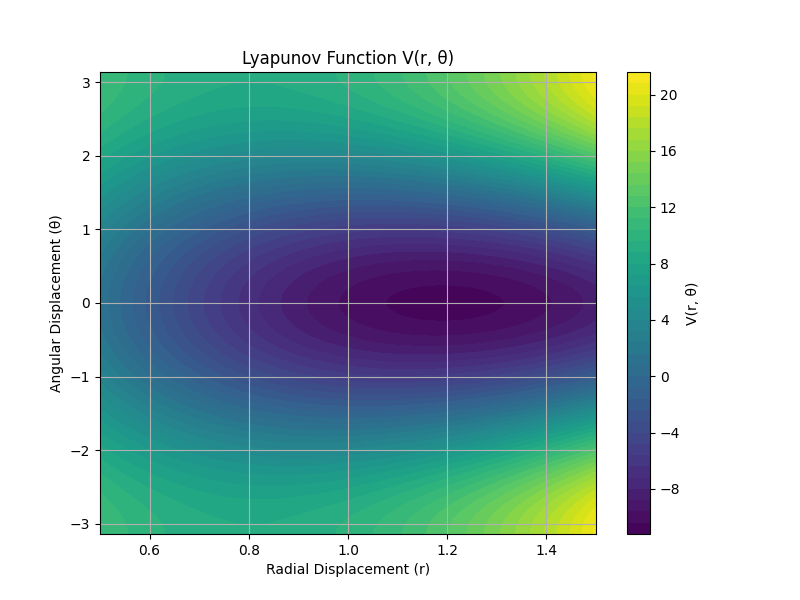
\includegraphics[width=0.8\textwidth]{lyapunov_function.png}
    \caption{Contour plot of the Lyapunov function \( V(r, \theta) \), representing the energy landscape of the system. The minima correspond to stable regions.}
    \label{fig:lyapunov_function}
\end{figure}

\subsubsection{Time Derivative of the Lyapunov Function}
The time derivative \( \dot{V}(r, \theta) \), shown in Figure~\ref{fig:lyapunov_derivative}, highlights regions of stability and instability. Regions where \( \dot{V} \leq 0 \) are stable, while regions where \( \dot{V} > 0 \) indicate energy growth and instability.

\begin{figure}[h!]
    \centering
    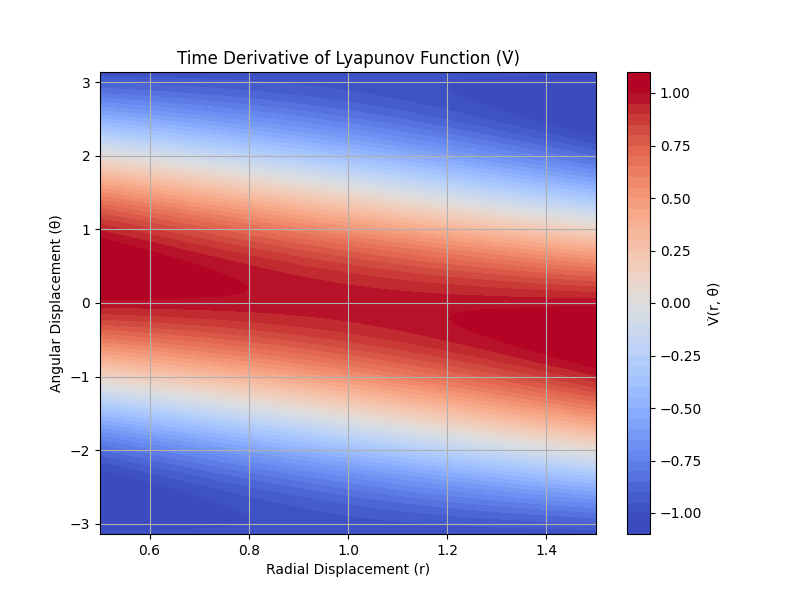
\includegraphics[width=0.8\textwidth]{lyapunov_derivative.png}
    \caption{Contour plot of the time derivative of the Lyapunov function \( \dot{V}(r, \theta) \). Stable regions (\( \dot{V} \leq 0 \)) are shown in cool colors, while unstable regions (\( \dot{V} > 0 \)) are in warm colors.}
    \label{fig:lyapunov_derivative}
\end{figure}

\subsection{Discussion}
The Lyapunov stability analysis provides the following insights:
\begin{itemize}
    \item The energy minima in the Lyapunov function \( V(r, \theta) \) correspond to stable equilibrium points of the system.
    \item Regions where \( \dot{V} > 0 \) indicate that the system's energy increases, leading to instability.
    \item The presence of stable and unstable regions demonstrates the nonlinear dynamics of the system, influenced by the coupling between radial and angular motion.
\end{itemize}
This analysis highlights the utility of the Lyapunov method in understanding stability in nonlinear systems.


\newpage

\section*{References}
\begin{enumerate}
    \item Morin, D. (2008). \textit{The Lagrangian Method}. Retrieved from: \url{https://scholar.harvard.edu/files/david-morin/files/cmchap6.pdf}
    \item Misra, I., \& Kumaran, V. (2017). \textit{Dynamics of a Magnetic Particle in an Oscillating Magnetic Field}. Physical Review Fluids. Retrieved from: \url{https://link.aps.org/doi/10.1103/PhysRevFluids.9.074303}
    \item LibreTexts. (2021). \textit{Magnetic Dipole Moment and Magnetic Dipole Media}. Retrieved from: \url{https://phys.libretexts.org/Bookshelves/Electricity_and_Magnetism/Essential_Graduate_Physics_-_Classical_Electrodynamics_(Likharev)/5.04:_Magnetic_Dipole_Moment_and_Magnetic_Dipole_Media}
    \item Physics Pages. (2018). \textit{Fields of an Oscillating Magnetic Dipole}. Retrieved from: \url{https://physicspages.com/pdf/Electrodynamics/Fields%20of%20an%20oscillating%20magnetic%20dipole.pdf}
    \item Wikipedia. (2023). \textit{Elastic Pendulum}. Retrieved from: \url{https://en.wikipedia.org/wiki/Elastic_pendulum}
    \item Press, W. H., Teukolsky, S. A., Vetterling, W. T., \& Flannery, B. P. (2007). \textit{Numerical Recipes: The Art of Scientific Computing} (3rd ed.). Cambridge University Press.
    \item Hairer, E., Nørsett, S. P., \& Wanner, G. (1993). \textit{Solving Ordinary Differential Equations I: Nonstiff Problems} (2nd ed.). Springer.
    \item Landau, R. H., Paez, M. J., \& Bordeianu, C. C. (2015). \textit{A Survey of Computational Physics: Introductory Computational Science}. Princeton University Press.
    \item Ascher, U. M., \& Petzold, L. R. (1998). \textit{Computer Methods for Ordinary Differential Equations and Differential-Algebraic Equations}. SIAM.
    \item Wikipedia contributors. (2023). \textit{Numerical methods for ordinary differential equations}. Retrieved from: \url{https://en.wikipedia.org/wiki/Numerical_methods_for_ordinary_differential_equations}
     \item Press, W. H., Teukolsky, S. A., Vetterling, W. T., \& Flannery, B. P. (2007). \textit{Numerical Recipes: The Art of Scientific Computing} (3rd ed.). Cambridge University Press.
    \item Hairer, E., Nørsett, S. P., \& Wanner, G. (1993). \textit{Solving Ordinary Differential Equations I: Nonstiff Problems} (2nd ed.). Springer.
    \item Landau, R. H., Paez, M. J., \& Bordeianu, C. C. (2015). \textit{A Survey of Computational Physics: Introductory Computational Science}. Princeton University Press.
    \item Ascher, U. M., \& Petzold, L. R. (1998). \textit{Computer Methods for Ordinary Differential Equations and Differential-Algebraic Equations}. SIAM.
    \item Wikipedia contributors. (2023). \textit{Numerical methods for ordinary differential equations}. Retrieved from: \url{https://en.wikipedia.org/wiki/Numerical_methods_for_ordinary_differential_equations}
\end{enumerate}

\end{document}
